\chapter{Molecular Orbitals of Diatomic Molecules}\label{ch:b2:diatomic-mos}

Pour liquid oxygen between the poles of a strong magnet and it is pulled
aside; liquid nitrogen falls straight through. The oxygen molecule carries
unpaired electrons, which a magnetic field attracts. Its Lewis structure,
\ce{O=O} with every electron paired, cannot say so. \omterm{def:b2:diatomic-mos:lcao}{Molecular orbitals},
built from the atomic orbitals of the previous chapter, place each electron
of a molecule in a level of its own: they account for the magnetism of
oxygen, for the strength and length of bonds, and for the energies needed to
ionise molecules --- and they lay the ground for the reactivity of the
chapters that follow.

\begin{recall}
\Cref{ch:b2:atomic-orbitals}: atomic orbitals, their shapes, signs and
energies. The Year 1 volume: Lewis structures, $\sigma$ and $\pi$ bonds as
descriptive notions, hybridisation and its limits, unpaired electrons and
radicals.
\end{recall}

\begin{omfigure}
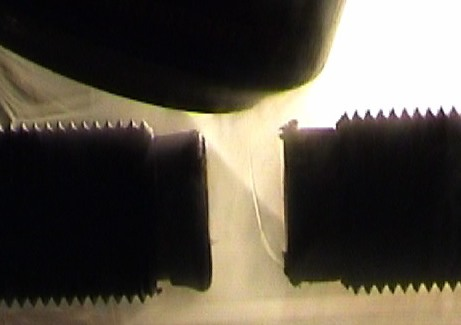
\includegraphics[width=0.42\linewidth]{images/book3/liquid-oxygen.jpg}

{\small A thin stream of liquid oxygen, falling between the poles of a strong
magnet, is drawn towards them and hangs as a bridge: the molecule is
\omterm{def:b2:diatomic-mos:magnetism}{paramagnetic}. (Photograph: Pieter Kuiper, public domain, Wikimedia Commons.)}
\end{omfigure}

\section{The LCAO method}

\begin{definition}[Molecular orbital]\label{def:b2:diatomic-mos:lcao}
A \emph{molecular orbital}\index{molecular orbital} is the \omterm{def:b2:atomic-orbitals:wavefunction}{wavefunction} of one
electron in a molecule, spread over all its nuclei. In the \emph{LCAO}\index{LCAO}
method (linear combination of atomic orbitals) it is written as a sum of atomic
orbitals of the atoms, $\psi = \sum_i c_i\varphi_i$, with coefficients chosen to
make the energy lowest.
\end{definition}

For two atoms A and B, each bringing one orbital, $\psi = c_A\varphi_A + c_B\varphi_B$.
The energy of an electron in $\psi$, minimised with respect to the coefficients,
brings in three numbers.

\begin{definition}[The integrals of the LCAO method]\label{def:b2:diatomic-mos:integrals}
For two real atomic orbitals $\varphi_A$, $\varphi_B$ and the energy operator $\hat H$
of an electron in the molecule:
\begin{itemize}
  \item the \emph{overlap integral}\index{overlap integral} $S = \int\varphi_A\varphi_B\,dV$
        measures how much the two orbitals occupy the same region ($S = 1$ for
        identical, superimposed orbitals);
  \item the \emph{Coulomb integral}\index{Coulomb integral} $\alpha_A = \int\varphi_A\hat
        H\varphi_A\,dV$ is the energy of an electron in $\varphi_A$ within the molecule,
        close to the atomic \omterm{def:b2:atomic-orbitals:orbital-energy}{orbital energy};
  \item the \emph{resonance integral}\index{resonance integral} $\beta = \int\varphi_A\hat
        H\varphi_B\,dV$, negative, measures the coupling of the two orbitals.
\end{itemize}
The energies $E$ of the \omterm{def:b2:diatomic-mos:lcao}{molecular orbitals} are the roots of the \emph{secular
determinant}\index{secular determinant}
\[
  \begin{vmatrix} \alpha_A - E & \beta - ES \\ \beta - ES & \alpha_B - E \end{vmatrix} = 0 .
\]
\end{definition}

The determinant comes from minimising $E = \int\psi\hat H\psi\,dV/\int\psi^2\,dV$
with respect to $c_A$ and $c_B$: the two conditions $\partial E/\partial c_A =
\partial E/\partial c_B = 0$ form a homogeneous linear system, which has a non-zero
solution only when its determinant vanishes. That variational step is admitted
here.

\begin{theorem}[Two identical orbitals]\label{thm:b2:diatomic-mos:homonuclear}
For $\alpha_A = \alpha_B = \alpha$, the two \omterm{def:b2:diatomic-mos:lcao}{molecular orbitals} are
\[
  E_+ = \frac{\alpha + \beta}{1 + S}, \quad \psi_+ = \frac{\varphi_A + \varphi_B}{\sqrt{2(1 + S)}} ;
  \qquad
  E_- = \frac{\alpha - \beta}{1 - S}, \quad \psi_- = \frac{\varphi_A - \varphi_B}{\sqrt{2(1 - S)}} .
\]
\end{theorem}

\begin{proof}
The determinant gives $(\alpha - E)^2 = (\beta - ES)^2$, so $\alpha - E = \pm(\beta - ES)$.
With the plus sign, $E(1 + S) = \alpha + \beta$; with the minus sign, $E(1 - S) = \alpha
- \beta$. Back in the linear system, $(\alpha - E)c_A + (\beta - ES)c_B = 0$ gives $c_B
= c_A$ for $E_+$ and $c_B = -c_A$ for $E_-$. Normalisation: $\int(\varphi_A \pm
\varphi_B)^2\,dV = 2 \pm 2S$.
\end{proof}

\begin{definition}[Bonding and antibonding orbitals]\label{def:b2:diatomic-mos:bonding}
A \emph{bonding orbital}\index{bonding orbital} lies below the atomic orbitals it
is made of: its electron density accumulates between the nuclei. An
\emph{antibonding orbital}\index{antibonding orbital} lies above them and has a
nodal plane between the nuclei. A \emph{nonbonding orbital}\index{nonbonding orbital}
keeps the energy of the atomic orbital, which finds no partner to
combine with.
\end{definition}

\begin{proposition}[The antibonding orbital rises more]\label{prop:b2:diatomic-mos:asymmetry}
For $S > 0$, the antibonding level is raised above $\alpha$ by more than the
bonding level is lowered below it.
\end{proposition}

\begin{proof}
$E_+ - \alpha = (\beta - \alpha S)/(1 + S)$ and $E_- - \alpha = -(\beta - \alpha S)/(1 - S)$.
The numerator $\beta - \alpha S$ is negative (the coupling dominates), and $1 - S < 1
+ S$: the second shift is larger in magnitude.
\end{proof}

With two electrons, as in \ce{H2}, both enter $\psi_+$ and the molecule is more
stable than the separate atoms. With four, as in \ce{He2}, two must enter $\psi_-$,
which costs more than $\psi_+$ gains: \ce{He2} is not bound.

\begin{omfigure}
\begin{MOdiagram}[names, labels]
  \atom[H]{left}{ 1s = {0;up} }
  \atom[H]{right}{ 1s = {0;up} }
  \molecule[\ce{H2}]{ 1sMO = {.75;pair} }
\end{MOdiagram}
\hspace{1.5cm}
\begin{MOdiagram}[names, labels]
  \atom[He]{left}{ 1s = {0;pair} }
  \atom[He]{right}{ 1s = {0;pair} }
  \molecule[\ce{He2}]{ 1sMO = {.75;pair,pair} }
\end{MOdiagram}

{\small \omterm{def:b2:diatomic-mos:lcao}{Molecular orbital} diagrams of \ce{H2} (\omterm{def:b2:diatomic-mos:bond-order}{bond order} 1) and \ce{He2} (\omterm{def:b2:diatomic-mos:bond-order}{bond
order} 0, not bound). Each box is a level holding at most two electrons of
opposite spins; dashed lines join each \omterm{def:b2:diatomic-mos:lcao}{molecular orbital} to the atomic orbitals
it is built from.}
\end{omfigure}

\section{Overlap and symmetry}

\begin{definition}[$\sigma$ and $\pi$ orbitals]\label{def:b2:diatomic-mos:sigma-pi}
A \emph{$\sigma$ orbital}\index{sigma orbital@$\sigma$ orbital} of a linear molecule is unchanged by any
rotation about the molecular axis: it has no nodal plane containing the axis. A
\emph{$\pi$ orbital}\index{pi orbital@$\pi$ orbital} changes sign under a rotation of $180^\circ$ about the
axis: it has one nodal plane containing the axis. An asterisk marks \omterm{def:b2:diatomic-mos:bonding}{antibonding
orbitals} ($\sigma^*$, $\pi^*$).
\end{definition}

\begin{proposition}[Zero overlap by symmetry]\label{prop:b2:diatomic-mos:symmetry}
Two orbitals of which one is symmetric and the other antisymmetric with respect
to a plane containing the molecular axis have zero overlap and zero \omterm{def:b2:diatomic-mos:integrals}{resonance
integral}: they do not combine.
\end{proposition}

\begin{proof}
Reflection in the plane leaves the space unchanged but turns the product
$\varphi_A\varphi_B$ into its opposite at the mirror point: the contributions of the
two halves of space to $\int\varphi_A\varphi_B\,dV$ cancel. The same holds for
$\int\varphi_A\hat H\varphi_B\,dV$, since $\hat H$ has the symmetry of the molecule.
\end{proof}

Two orbitals interact strongly when they have the same symmetry (non-zero
overlap), overlap well, and lie at close energies. A 1s orbital of one atom and a
$2\mathrm p_x$ of the other ($x$ perpendicular to the axis) never combine;
$2\mathrm p_z$ orbitals (along the axis) give $\sigma$ orbitals; $2\mathrm p_x$ and
$2\mathrm p_y$ give two pairs of $\pi$ orbitals of equal energies.

\begin{omfigure}
\begin{tikzpicture}[font=\small]
  % sigma 1s
  \pic at (0,0) {oms={0.85}}; \pic at (0.7,0) {oms={0.85}};
  \node at (0.35,-0.75) {$\sigma_{1s}$};
  \pic at (2.2,0) {oms={0.85}}; \pic at (2.9,0) {oms={-0.85}};
  \node at (2.55,-0.75) {$\sigma^*_{1s}$};
  % sigma 2p
  \pic at (4.6,0) {omp={-1}{0}}; \pic at (5.6,0) {omp={1}{0}};
  \node at (5.1,-0.75) {$\sigma_{2p}$};
  \pic at (7.4,0) {omp={-1}{0}}; \pic at (8.6,0) {omp={-1}{0}};
  \node at (8.0,-0.75) {$\sigma^*_{2p}$};
  % pi 2p
  \pic at (10.2,0) {omp={1}{90}}; \pic at (10.9,0) {omp={1}{90}};
  \node at (10.55,-0.95) {$\pi_{2p}$};
  \pic at (12.2,0) {omp={1}{90}}; \pic at (12.9,0) {omp={-1}{90}};
  \node at (12.55,-0.95) {$\pi^*_{2p}$};
  \draw[black!40, dashed] (-0.6,0) -- (13.4,0);
\end{tikzpicture}

{\small \omterm{def:b2:diatomic-mos:lcao}{Molecular orbitals} of a homonuclear diatomic, schematic (the molecular
axis is horizontal and dashed). In-phase combinations (bonding) gather the
same colour between the nuclei; out-of-phase combinations (antibonding) put a
nodal plane between them. $\sigma$ orbitals are symmetric about the axis; each $\pi$
orbital has the axis in its nodal plane.}
\end{omfigure}

\section{Homonuclear diatomics of period 2}

With the 2s and 2p orbitals of two atoms of period 2, eight \omterm{def:b2:diatomic-mos:lcao}{molecular orbitals}
form: $\sigma_{2s}$, $\sigma^*_{2s}$, $\sigma_{2p}$, two $\pi_{2p}$, two $\pi^*_{2p}$,
$\sigma^*_{2p}$.

\begin{proposition}[s--p mixing]\label{prop:b2:diatomic-mos:sp-mixing}
For \ce{O2} and \ce{F2} the order is $\sigma_{2s} < \sigma^*_{2s} < \sigma_{2p} < \pi_{2p} <
\pi^*_{2p} < \sigma^*_{2p}$. For \ce{Li2} to \ce{N2}, whose 2s and 2p levels are close,
the $\sigma$ orbitals made from 2s and $2\mathrm p_z$ mix: $\sigma_{2p}$ is pushed up above
$\pi_{2p}$.
\end{proposition}

\begin{proof}[Argument]
The $\sigma_{2s}$ and $\sigma_{2p}$ orbitals have the same symmetry and can combine with
each other. Two levels of the same symmetry repel (\cref{thm:b2:diatomic-mos:heteronuclear}
below): $\sigma_{2s}$ goes down, $\sigma_{2p}$ goes up, the more so as they are close. The
2s--2p gap grows along the period, so the effect is large on the left and small for
oxygen and fluorine. The crossing between nitrogen and oxygen is admitted from the
measured photoelectron spectra.
\end{proof}

\begin{definition}[Bond order]\label{def:b2:diatomic-mos:bond-order}
The \emph{bond order}\index{bond order} of a diatomic molecule is $b = (n_b -
n_a)/2$, where $n_b$ and $n_a$ are the numbers of electrons in bonding and
\omterm{def:b2:diatomic-mos:bonding}{antibonding orbitals}.
\end{definition}

\begin{proposition}[Bond order and bond]\label{prop:b2:diatomic-mos:bond-order}
Between atoms of the same pair of elements, a higher \omterm{def:b2:diatomic-mos:bond-order}{bond order} goes with a
shorter and stronger bond; a \omterm{def:b2:diatomic-mos:bond-order}{bond order} of zero means no bond.
\end{proposition}

\begin{proof}[Argument]
Each bonding electron adds density between the nuclei and lowers the energy;
each antibonding electron removes it and raises the energy by at least as much
(\cref{prop:b2:diatomic-mos:asymmetry}). The net number of bonding pairs measures
the binding. The comparison is meaningful only for similar atoms: \ce{Li2} has
\omterm{def:b2:diatomic-mos:bond-order}{bond order} 1 like \ce{F2}, but its 2s orbitals are far larger.
\end{proof}

\begin{definition}[Paramagnetic and diamagnetic]\label{def:b2:diatomic-mos:magnetism}
A substance is \emph{paramagnetic}\index{paramagnetic} if its molecules have
unpaired electrons: it is drawn into a magnetic field. It is
\emph{diamagnetic}\index{diamagnetic} if all its electrons are paired: it is
weakly pushed out of the field.
\end{definition}

\begin{omfigure}
\begin{MOdiagram}[names, labels, style=square, distance=4.2cm, labels-fs=\scriptsize]
  \atom[N]{left}{ 2s = {0;pair}, 2p = {3.5;up,up,up} }
  \atom[N]{right}{ 2s = {0;pair}, 2p = {3.5;up,up,up} }
  \molecule[\ce{N2}]{ 2sMO = {.7;pair,pair}, 2pMO = {0.4/2.5,1.4;pair,pair,pair} }
\end{MOdiagram}
\hfill
\begin{MOdiagram}[names, labels, style=square, distance=4.2cm, labels-fs=\scriptsize]
  \atom[O]{left}{ 2s = {0;pair}, 2p = {3.5;pair,up,up} }
  \atom[O]{right}{ 2s = {0;pair}, 2p = {3.5;pair,up,up} }
  \molecule[\ce{O2}]{ 2sMO = {.7;pair,pair}, 2pMO = {1.8,.8;pair,pair,pair,up,up} }
\end{MOdiagram}

{\small Valence \omterm{def:b2:diatomic-mos:lcao}{molecular orbital} diagrams of \ce{N2} (left, with s--p mixing:
$\sigma_{2p}$ above $\pi_{2p}$) and \ce{O2} (right). Nitrogen: \omterm{def:b2:diatomic-mos:bond-order}{bond order}
$(8 - 2)/2 = 3$, all electrons paired. Oxygen: \omterm{def:b2:diatomic-mos:bond-order}{bond order} $(8 - 4)/2 = 2$, with two
unpaired electrons in the two $\pi^*$ orbitals (Hund's rule): \ce{O2} is
\omterm{def:b2:diatomic-mos:magnetism}{paramagnetic}. The diagrams take $x$ as the molecular axis, hence the labels
$2\sigma_x$, $2\pi_y$, $2\pi_z$.}
\end{omfigure}

\begin{method}[Building and filling an MO diagram]\label{met:b2:diatomic-mos:build-diagram}
\begin{enumerate}
  \item Place the valence atomic orbitals of each atom at their energies, the more
        electronegative atom lower.
  \item Combine orbitals of the same symmetry: each pair gives one \omterm{def:b2:diatomic-mos:bonding}{bonding orbital}
        below and one \omterm{def:b2:diatomic-mos:bonding}{antibonding orbital} above; an orbital without a partner stays
        nonbonding.
  \item For period 2 homonuclear molecules, use the order with $\sigma_{2p}$ above
        $\pi_{2p}$ up to nitrogen, below it from oxygen on.
\end{enumerate}
\end{method}

\begin{method}[Reading a filled diagram]\label{met:b2:diatomic-mos:fill}
\begin{enumerate}
  \item Count the valence electrons (add one for each negative charge, remove one
        for each positive charge).
  \item Fill from the bottom, two per orbital, with Hund's rule for degenerate
        levels.
  \item \omterm{def:b2:diatomic-mos:bond-order}{Bond order} $(n_b - n_a)/2$; unpaired electrons give paramagnetism.
  \item The highest occupied level is the one ionised first.
\end{enumerate}
\end{method}

\begin{omfigure}
\small
\renewcommand{\arraystretch}{1.15}
\begin{tabular}{lcccccc}
 & \ce{Li2} & \ce{C2} & \ce{N2} & \ce{O2} & \ce{F2} & \ce{NO} \\ \hline
valence electrons & 2 & 8 & 10 & 12 & 14 & 11 \\
\omterm{def:b2:diatomic-mos:bond-order}{bond order} & 1 & 2 & 3 & 2 & 1 & 2.5 \\
unpaired electrons & 0 & 0 & 0 & 2 & 0 & 1 \\
bond length $r_e$ (pm) & 267.3 & 124.3 & 109.8 & 120.8 & 141.2 & 115.1 \\
$D_0$ (\unit{eV}) & 1.04 & 6.15 & 9.76 & 5.12 & 1.60 & 6.51 \\
\end{tabular}

\smallskip
{\small Period-2 diatomics: \omterm{def:b2:diatomic-mos:bond-order}{bond orders} from the MO diagrams; bond lengths from
spectroscopy, dissociation energies $D_0$ from tabulated enthalpies of formation
at \qty{0}{K}, $D_0 = \Delta_f H_0(\mathrm A) + \Delta_f H_0(\mathrm B) - \Delta_f
H_0(\mathrm{AB})$.}
% ledger: re:Li2, re:C2, re:N2, re:O2, re:F2, re:NO, janafH0:Li, janafH0:Li2, janafH0:C, janafH0:C2, janafH0:N, janafH0:O, janafH0:F, janafH0:NO
\end{omfigure}

\section{Heteronuclear diatomics}

\begin{theorem}[Two orbitals of different energies]\label{thm:b2:diatomic-mos:heteronuclear}
For $\alpha_A > \alpha_B$ (B more electronegative), $S$ neglected, $\bar\alpha = (\alpha_A
+ \alpha_B)/2$ and $\Delta = \alpha_A - \alpha_B$:
\[
  E_\mp = \bar\alpha \mp \sqrt{\Delta^2/4 + \beta^2} .
\]
The \omterm{def:b2:diatomic-mos:bonding}{bonding orbital} (lower) has its larger coefficient on B, the \omterm{def:b2:diatomic-mos:bonding}{antibonding
orbital} on A; when $\Delta \gg |\beta|$, $E_- \approx \alpha_B - \beta^2/\Delta$ and $E_+
\approx \alpha_A + \beta^2/\Delta$.
\end{theorem}

\begin{proof}
With $S = 0$ the energies are the eigenvalues of $\begin{pmatrix}\alpha_A & \beta \\
\beta & \alpha_B\end{pmatrix}$: $(\alpha_A - E)(\alpha_B - E) = \beta^2$, whose roots are
$\bar\alpha \pm \sqrt{\Delta^2/4 + \beta^2}$. For the lower root, $(\alpha_B - E_-)c_B = -\beta
c_A$; $\alpha_B - E_- = \sqrt{\Delta^2/4 + \beta^2} - \Delta/2$ is smaller than $|\beta|$, so
$|c_A| < |c_B|$. For $\Delta \gg |\beta|$, $\sqrt{\Delta^2/4 + \beta^2} \approx \Delta/2 +
\beta^2/\Delta$.
\end{proof}

\begin{omfigure}
\begin{tikzpicture}
\begin{axis}[width=0.55\linewidth, height=6cm, xmin=0, xmax=8, ymin=-5, ymax=5,
  axis x line=bottom, axis y line=left, xlabel={$\Delta/|\beta|$}, ylabel={$E/|\beta|$},
  tick label style={font=\small}, label style={font=\small}]
\addplot[omThm, thick] table[x=d, y=Ehigh] {figdata/out/bachelor-2-two-level-a.dat};
\addplot[omDef, thick] table[x=d, y=Elow] {figdata/out/bachelor-2-two-level-a.dat};
\addplot[black!50, densely dotted] table[x=d, y=aA] {figdata/out/bachelor-2-two-level-a.dat};
\addplot[black!50, densely dotted] table[x=d, y=aB] {figdata/out/bachelor-2-two-level-a.dat};
\addplot[omThm, dashed] table[x=d, y=Phigh] {figdata/out/bachelor-2-two-level-a-pert.dat};
\addplot[omDef, dashed] table[x=d, y=Plow] {figdata/out/bachelor-2-two-level-a-pert.dat};
\node[font=\scriptsize, black!60, anchor=north west] at (axis cs:5.5,2.6) {$\alpha_A$};
\node[font=\scriptsize, black!60, anchor=south west] at (axis cs:5.5,-2.6) {$\alpha_B$};
\node[font=\scriptsize, omThm, anchor=south east] at (axis cs:3.2,2.2) {antibonding};
\node[font=\scriptsize, omDef, anchor=north east] at (axis cs:3.2,-2.2) {bonding};
\end{axis}
\end{tikzpicture}

{\small Two interacting levels. As the gap $\Delta$ between the atomic orbitals grows,
the molecular levels (solid) approach the atomic ones (dotted): the stabilisation
$\beta^2/\Delta$ of the perturbative limit (dashed) becomes small. At $\Delta = 0$ the
splitting is $2|\beta|$.}
\end{omfigure}

In hydrogen fluoride, the 1s orbital of hydrogen meets the far lower 2p orbitals
of fluorine. Only $2\mathrm p_z$, along the axis, has the right symmetry: it forms
a $\sigma$ \omterm{def:b2:diatomic-mos:bonding}{bonding orbital} weighted on fluorine, and a $\sigma^*$ weighted on
hydrogen. The $2\mathrm p_x$ and $2\mathrm p_y$ orbitals of fluorine stay
nonbonding: they are its lone pairs. The bond is polarised towards fluorine.

Carbon monoxide has the ten valence electrons of \ce{N2} and a similar diagram,
but the oxygen orbitals lie lower. Its \omterm{def:b2:diatomic-mos:bonding}{bonding orbitals} are weighted on oxygen;
its highest occupied orbital, a $\sigma$ orbital weighted on carbon, is a lone pair
on carbon. Carbon monoxide therefore binds metals through carbon
(\cref{ch:b2:coordination-complexes}).

\begin{omfigure}
\begin{tikzpicture}[font=\small]
  % CO schematic: C left (higher), O right (lower)
  \pic (c2s) at (0,0.6) {omlevel={ud}{0.8}}; \node[left] at (-0.5,0.6) {2s};
  \pic (c2p1) at (-0.45,2.6) {omlevel={u}{0.4}}; \pic (c2p2) at (0,2.6) {omlevel={u}{0.4}}; \pic (c2p3) at (0.45,2.6) {omlevel={empty}{0.4}};
  \node[left] at (-0.75,2.6) {2p};
  \node at (0,-0.6) {C};
  \pic (o2s) at (6,-1.2) {omlevel={ud}{0.8}}; \node[right] at (6.5,-1.2) {2s};
  \pic (o2p1) at (5.55,1.4) {omlevel={ud}{0.4}}; \pic (o2p2) at (6,1.4) {omlevel={u}{0.4}}; \pic (o2p3) at (6.45,1.4) {omlevel={u}{0.4}};
  \node[right] at (6.75,1.4) {2p};
  \node at (6,-2.2) {O};
  % MOs
  \pic (m1) at (3,-1.8) {omlevel={ud}{0.8}};
  \pic (m2) at (3,-0.2) {omlevel={ud}{0.8}};
  \pic (m3a) at (2.75,0.9) {omlevel={ud}{0.45}}; \pic (m3b) at (3.25,0.9) {omlevel={ud}{0.45}};
  \pic (m4) at (3,1.9) {omlevel={ud}{0.8}};
  \pic (m5a) at (2.75,3.3) {omlevel={empty}{0.45}}; \pic (m5b) at (3.25,3.3) {omlevel={empty}{0.45}};
  \pic (m6) at (3,4.4) {omlevel={empty}{0.8}};
  \draw[omcorr, densely dashed] (c2s-r) -- (m1-l) (o2s-l) -- (m1-r);
  \draw[omcorr, densely dashed] (c2s-r) -- (m2-l) (o2s-l) -- (m2-r);
  \draw[omcorr, densely dashed] (c2p3-r) -- (m3a-l) (o2p1-l) -- (m3b-r);
  \draw[omcorr, densely dashed] (c2p3-r) -- (m4-l) (o2p1-l) -- (m4-r);
  \draw[omcorr, densely dashed] (c2p3-r) -- (m5a-l) (o2p1-l) -- (m5b-r);
  \draw[omcorr, densely dashed] (c2p3-r) -- (m6-l) (o2p1-l) -- (m6-r);
  \node[omsymlabel, below=0.17cm, inner sep=0.5pt] at (m1-c) {$\sigma$};
  \node[omsymlabel, below=0.17cm, inner sep=0.5pt] at (m2-c) {$\sigma$};
  \node[omsymlabel, below=0.17cm, inner sep=0.5pt] at (3,0.9) {$\pi$};
  \node[omsymlabel, below=0.24cm, inner sep=0.5pt] at (m4-c) {$\sigma$ (C lone pair)};
  \node[omsymlabel, below=0.05cm, inner sep=0.5pt] at (3,3.3) {$\pi^*$};
  \node[omsymlabel, below=0.05cm, inner sep=0.5pt] at (m6-c) {$\sigma^*$};
  \node at (3,-2.6) {CO};
\end{tikzpicture}

{\small Valence orbitals of carbon monoxide, schematic: the oxygen orbitals lie
lower than those of carbon. \omterm{def:b2:diatomic-mos:bond-order}{Bond order} 3 as in \ce{N2}; the highest occupied
orbital is a $\sigma$ orbital weighted on carbon, its lone pair.}
\end{omfigure}

\begin{history}[Hund and Mulliken]
\begin{minipage}[t]{0.27\linewidth}
\vspace{0pt}
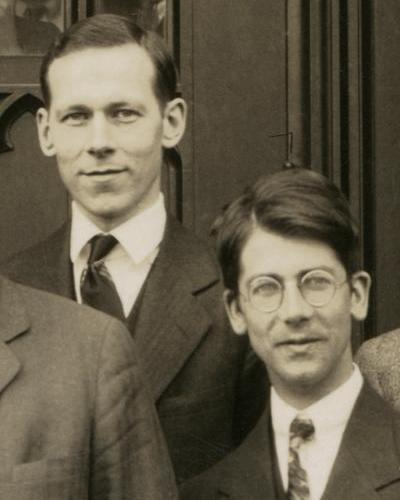
\includegraphics[width=\linewidth]{images/book3/mulliken-hund.jpg}
\end{minipage}\hfill
\begin{minipage}[t]{0.69\linewidth}
\vspace{0pt}
Between 1926 and 1932 Friedrich Hund and Robert Mulliken interpreted the spectra
of diatomic molecules by assigning each electron to an orbital of the whole
molecule, classified by its symmetry about the axis. The words $\sigma$, $\pi$,
bonding and antibonding, and the orbital diagrams of this chapter come from their
work; Mulliken received the Nobel Prize in Chemistry in 1966. The photograph shows
Mulliken (left) and Hund in Chicago in 1929. (Photograph: GFHund, CC BY 3.0,
Wikimedia Commons.)
\end{minipage}
\end{history}

\section{Ionisation and bond strength}

Removing an electron from a \omterm{def:b2:diatomic-mos:bonding}{bonding orbital} weakens the bond; removing it from
an \omterm{def:b2:diatomic-mos:bonding}{antibonding orbital} strengthens it. The dissociation energies of the ions
follow from a thermochemical cycle: for $\mathrm{AB}^+ \to \mathrm A + \mathrm B^+$,
\[
  D_0(\mathrm{AB}^+) = D_0(\mathrm{AB}) + I(\mathrm B) - I(\mathrm{AB}) ,
\]
B being the atom of lower ionisation energy.

\begin{example}[Nitrogen and oxygen ions]\label{ex:b2:diatomic-mos:ions}
\ce{N2} ($I = \qty{15.58}{eV}$) loses a bonding electron: $D_0(\ce{N2+}) = 9.76 + 14.53 -
15.58 = \qty{8.71}{eV}$, weaker than \ce{N2}. \ce{O2} ($I = \qty{12.07}{eV}$) loses a
$\pi^*$ electron: $D_0(\ce{O2+}) = 5.12 + 13.62 - 12.07 = \qty{6.66}{eV}$, stronger than \ce{O2},
in line with \omterm{def:b2:diatomic-mos:bond-order}{bond orders} 2.5 and 2.5 against 3 and 2.
% ledger: ie:N2, ie:N, ie:O2, ie:O, janafH0:N, janafH0:O
\end{example}

\section{Exercises}

\begin{exercise}[$\star$]\label{exo:b2:diatomic-mos:1}
For two hydrogen 1s orbitals take $\alpha = \qty{-13.6}{eV}$, $\beta = \qty{-9.0}{eV}$ and
$S = 0.60$ (exercise data). Compute $E_+$ and $E_-$, then the energy of the two
electrons of \ce{H2} compared with two separate atoms.
\end{exercise}

\begin{exercise}[$\star$]\label{exo:b2:diatomic-mos:2}
Give the \omterm{def:b2:diatomic-mos:bond-order}{bond orders} of \ce{He2}, \ce{He2+}, \ce{Li2} and \ce{B2} (with s--p
mixing).
\end{exercise}

\begin{exercise}[$\star$]\label{exo:b2:diatomic-mos:3}
Which of \ce{B2}, \ce{C2}, \ce{N2}, \ce{O2}, \ce{F2} are \omterm{def:b2:diatomic-mos:magnetism}{paramagnetic}?
\end{exercise}

\begin{exercise}[$\star$]\label{exo:b2:diatomic-mos:4}
The molecular axis is $z$. Which pairs among (1s, $2\mathrm p_z$), (1s,
$2\mathrm p_x$), ($2\mathrm p_x$, $2\mathrm p_x$), ($2\mathrm p_x$, $2\mathrm p_y$),
(2s, $2\mathrm p_z$) have non-zero overlap?
\end{exercise}

\begin{exercise}[$\star\star$]\label{exo:b2:diatomic-mos:5}
Predict whether \ce{N2+} has a longer or shorter bond than \ce{N2}, and check with
its dissociation energy computed in the chapter.
\end{exercise}

\begin{exercise}[$\star\star$]\label{exo:b2:diatomic-mos:6}
Carbon monoxide and \ce{N2} are isoelectronic. Explain why the \omterm{def:b2:diatomic-mos:bonding}{bonding orbitals} of
CO are weighted on oxygen and why its highest occupied orbital is a lone pair on
carbon.
\end{exercise}

\begin{exercise}[$\star\star$]\label{exo:b2:diatomic-mos:7}
In HF, which orbitals of fluorine interact with the 1s of hydrogen, and which stay
nonbonding? Draw the diagram.
\end{exercise}

\begin{exercise}[$\star\star$]\label{exo:b2:diatomic-mos:8}
With $\alpha_A = \qty{-10}{eV}$, $\alpha_B = \qty{-14}{eV}$ and $\beta = \qty{-3.0}{eV}$
(exercise data, $S$ neglected), compute the two energies and the weight $c_B^2$ of
the \omterm{def:b2:diatomic-mos:bonding}{bonding orbital} on B.
\end{exercise}

\begin{exercise}[$\star\star$]\label{exo:b2:diatomic-mos:9}
With s--p mixing, show that \ce{C2} has \omterm{def:b2:diatomic-mos:bond-order}{bond order} 2 made of two $\pi$ bonds and no
$\sigma_{2p}$ bond.
\end{exercise}

\begin{exercise}[$\star\star\star$]\label{exo:b2:diatomic-mos:10}
Give the \omterm{def:b2:diatomic-mos:bond-order}{bond orders} of NO and \ce{NO+}. From $D_0(\ce{NO}) = \qty{6.51}{eV}$, $I(\ce{NO}) =
\qty{9.26}{eV}$ and $I(\ce{O}) = \qty{13.62}{eV}$, compute $D_0(\ce{NO+})$ for $\ce{NO+} \to
\ce{N} + \ce{O+}$, and comment.
\end{exercise}

\begin{exercise}[$\star\star\star$]\label{exo:b2:diatomic-mos:11}
Show that $E_+ + E_- = 2(\alpha - \beta S)/(1 - S^2)$, and that it exceeds $2\alpha$ when
$\beta < \alpha S < 0$. Deduce why two filled orbitals repel (four-electron
destabilisation).
\end{exercise}

\begin{exercise}[$\star\star\star$]\label{exo:b2:diatomic-mos:12}
Order \ce{O2+}, \ce{O2}, \ce{O2-}, \ce{O2^2-} by \omterm{def:b2:diatomic-mos:bond-order}{bond order}, bond length and bond
strength. Which ion is found in hydrogen peroxide, and which in the yellow
compound \ce{KO2}?
\end{exercise}

\section{Problem: Oxygen and Its Ions}

\begin{problem}[{Weekend problem --- the molecular orbital diagram of dioxygen,
the bond orders and magnetism of its ions, ionisation and the strength of the
bond, and the two ways of pairing the $\pi^*$ electrons}]
\label{pb:b2:diatomic-mos:1}
Data: $I(\ce{O}) = \qty{13.62}{eV}$, $I(\ce{O2}) = \qty{12.07}{eV}$, $I(\ce{N}) =
\qty{14.53}{eV}$, $I(\ce{N2}) = \qty{15.58}{eV}$; $\Delta_f H_0$ at \qty{0}{K}
(\unit{kJ/mol}): \ce{O} 246.79, \ce{N} 470.82; $r_e$: \ce{O2} \qty{120.8}{pm}, \ce{N2}
\qty{109.8}{pm}; $1\ \unit{eV} = \qty{96.485}{kJ/mol}$.
% ledger: ie:O, ie:O2, ie:N, ie:N2, janafH0:O, janafH0:N, re:O2, re:N2

\medskip
\noindent\textbf{Part I --- Dioxygen.}
\begin{enumerate}
  \item How many valence electrons does \ce{O2} have?
  \item Draw its valence MO diagram (no s--p mixing) and fill it.
  \item Compute its \omterm{def:b2:diatomic-mos:bond-order}{bond order}.
  \item How many unpaired electrons? Is \ce{O2} \omterm{def:b2:diatomic-mos:magnetism}{paramagnetic}?
  \item Why does the Lewis structure fail here?
  \item Compute $D_0(\ce{O2})$ in \unit{eV}.
\end{enumerate}

\medskip
\noindent\textbf{Part II --- The ions.}
\begin{enumerate}[resume]
  \item Give the configuration and \omterm{def:b2:diatomic-mos:bond-order}{bond order} of \ce{O2+}.
  \item Same for the superoxide ion \ce{O2-}.
  \item Same for the peroxide ion \ce{O2^2-}.
  \item Give the number of unpaired electrons of each ion.
  \item Order \ce{O2+}, \ce{O2}, \ce{O2-}, \ce{O2^2-} by predicted bond length.
  \item Which ion has an O--O single bond, like hydrogen peroxide?
  \item Which of the four species are \omterm{def:b2:diatomic-mos:magnetism}{paramagnetic}?
\end{enumerate}

\medskip
\noindent\textbf{Part III --- Ionisation.}
\begin{enumerate}[resume]
  \item From which orbital does the electron leave when \ce{O2} is ionised?
  \item Why is $I(\ce{O2})$ lower than $I(\ce{O})$?
  \item Show that $D_0(\ce{O2+}) = D_0(\ce{O2}) + I(\ce{O}) - I(\ce{O2})$ and compute it.
  \item Compare with $D_0(\ce{O2})$ and explain.
  \item Compute $D_0(\ce{N2})$ and $D_0(\ce{N2+})$ in the same way.
  \item Why is $I(\ce{N2})$ higher than $I(\ce{N})$?
  \item Summarise: when does ionisation strengthen a bond?
\end{enumerate}

\medskip
\noindent\textbf{Part IV --- The $\pi^*$ electrons.}
\begin{enumerate}[resume]
  \item In the ground state the two $\pi^*$ electrons occupy two different orbitals with
        parallel spins. Which rule says so?
  \item Describe a state in which both occupy the same $\pi^*$ orbital.
  \item Why is that state higher in energy?
  \item What are its \omterm{def:b2:diatomic-mos:bond-order}{bond order} and its magnetism?
  \item State the \omterm{def:b2:diatomic-mos:bond-order}{bond order} of \ce{O2+} and its dissociation energy.
\end{enumerate}
\end{problem}
